\chapter{Additional Team Negotiation Results} \label{ap6:team}

This appendix presents supplementary material for the team-negotiation results of Section~\ref{sec:results-team}. Section~\ref{ap6:deltas} reports the team-versus-default win-rate and payoff deltas for all thirty-six configurations (game $\times$ seat $\times$ composition $\times$ opponent), and Section~\ref{ap6:dynamics} examines the internal deliberation, showing how member agreement builds over discussion rounds and which drafts the consensus rule selects.

\section{Per-Configuration Deltas} \label{ap6:deltas}

Figure~\ref{fig:team-delta-winrate-heatmap} gives the team-minus-default win-rate delta for every configuration, and Figure~\ref{fig:team-delta-payoff-heatmap} its payoff counterpart.

\begin{figure}[ht]
    \centering
    
\includegraphics[width=0.85\linewidth]{figures/results/team/team_delta_winrate_heatmap.png}
    \caption{Team-minus-default win-rate delta for every configuration. Most are close to
    zero; none reach confidence-interval separation in win rate.}
    \label{fig:team-delta-winrate-heatmap}
\end{figure}

\begin{figure}[ht]
    \centering
    
\includegraphics[width=0.85\linewidth]{figures/results/team/team_delta_payoff_heatmap.png}
    \caption{Team-minus-default payoff delta for every configuration. The few separated gains
    are concentrated in first-player seats, led by the heterogeneous team in BuySell and
    Ultimatum.}
    \label{fig:team-delta-payoff-heatmap}
\end{figure}

\section{Deliberation and Consensus} \label{ap6:dynamics}

Figure~\ref{fig:discussion-dynamics} tracks how member agreement and revision evolve across the discussion rounds. Figure~\ref{fig:hetero-family-consensus} reports move authorship in heterogeneous teams, and Figure~\ref{fig:consensus-robustness} probes the consensus rule on homogeneous teams to separate slate-position effects from draft-length effects.

\begin{figure}[ht]
    \centering
    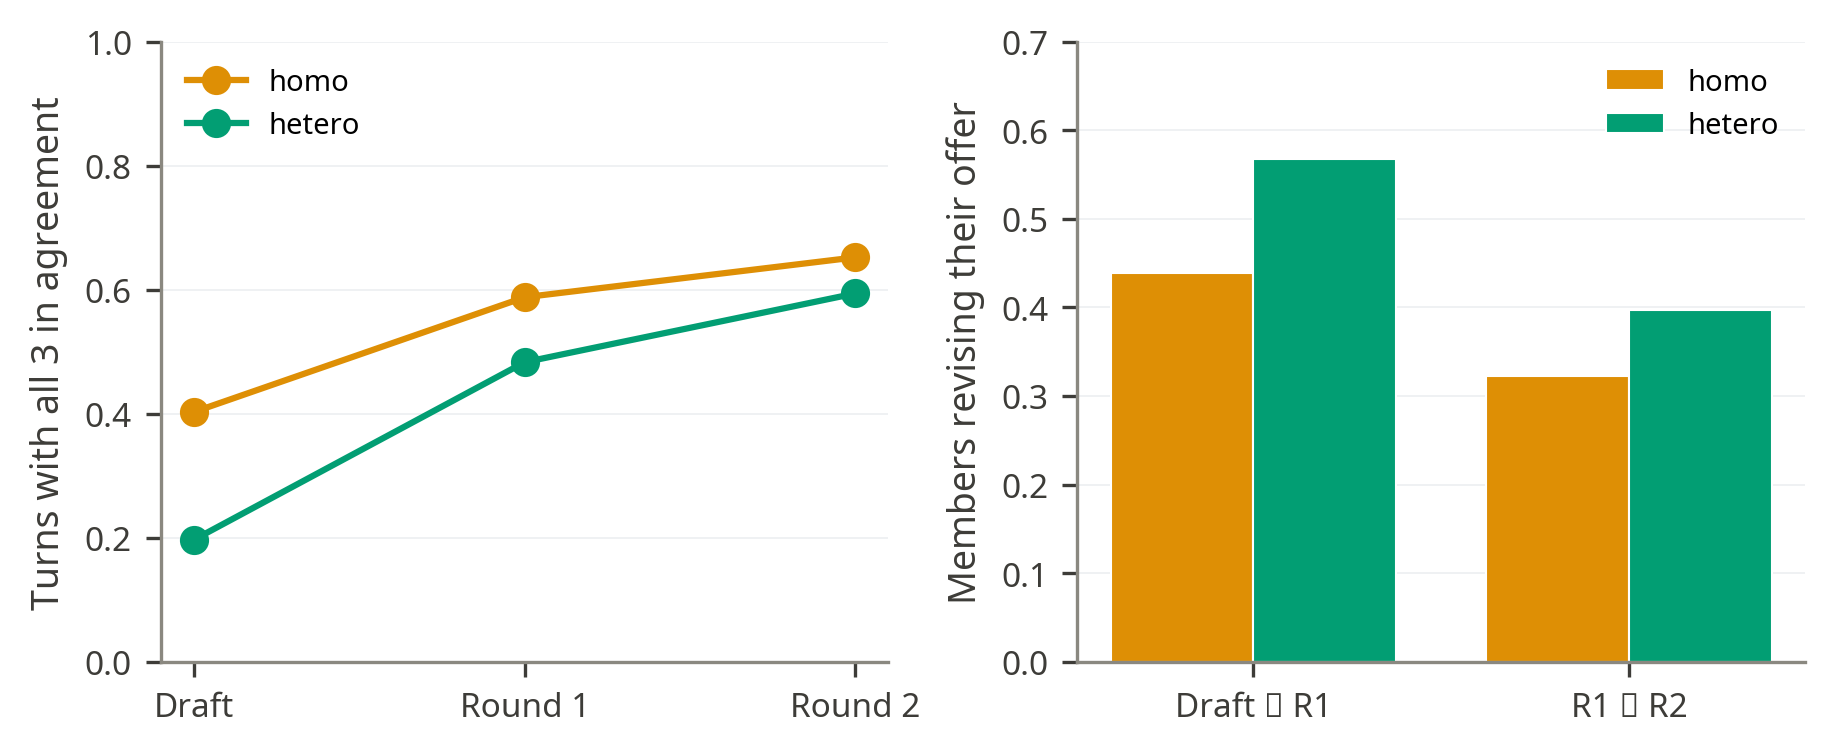
\includegraphics[width=0.95\linewidth]{figures/results/team/discussion_dynamics.png}
    \caption{Member deliberation over rounds. Left: share of turns on which all three members
    propose the same offer, which rises across rounds for both compositions. Right: share of
    members revising their offer at each transition; most revision happens in the first round.}
    \label{fig:discussion-dynamics}
\end{figure}

\begin{figure}[ht]
    \centering
    
\includegraphics[width=0.95\linewidth]{figures/results/team/hetero_family_consensus_authorship.png}
    \caption{Chosen move authorship in heterogeneous teams. Left: each family's share of
    selected moves; Mistral authors about $80\%$ of the team's committed moves. Right:
    selected-move authorship share by game, showing Mistral's dominance is consistent
    across all three games.}
    \label{fig:hetero-family-consensus}
\end{figure}

\begin{figure}[ht]
    \centering
    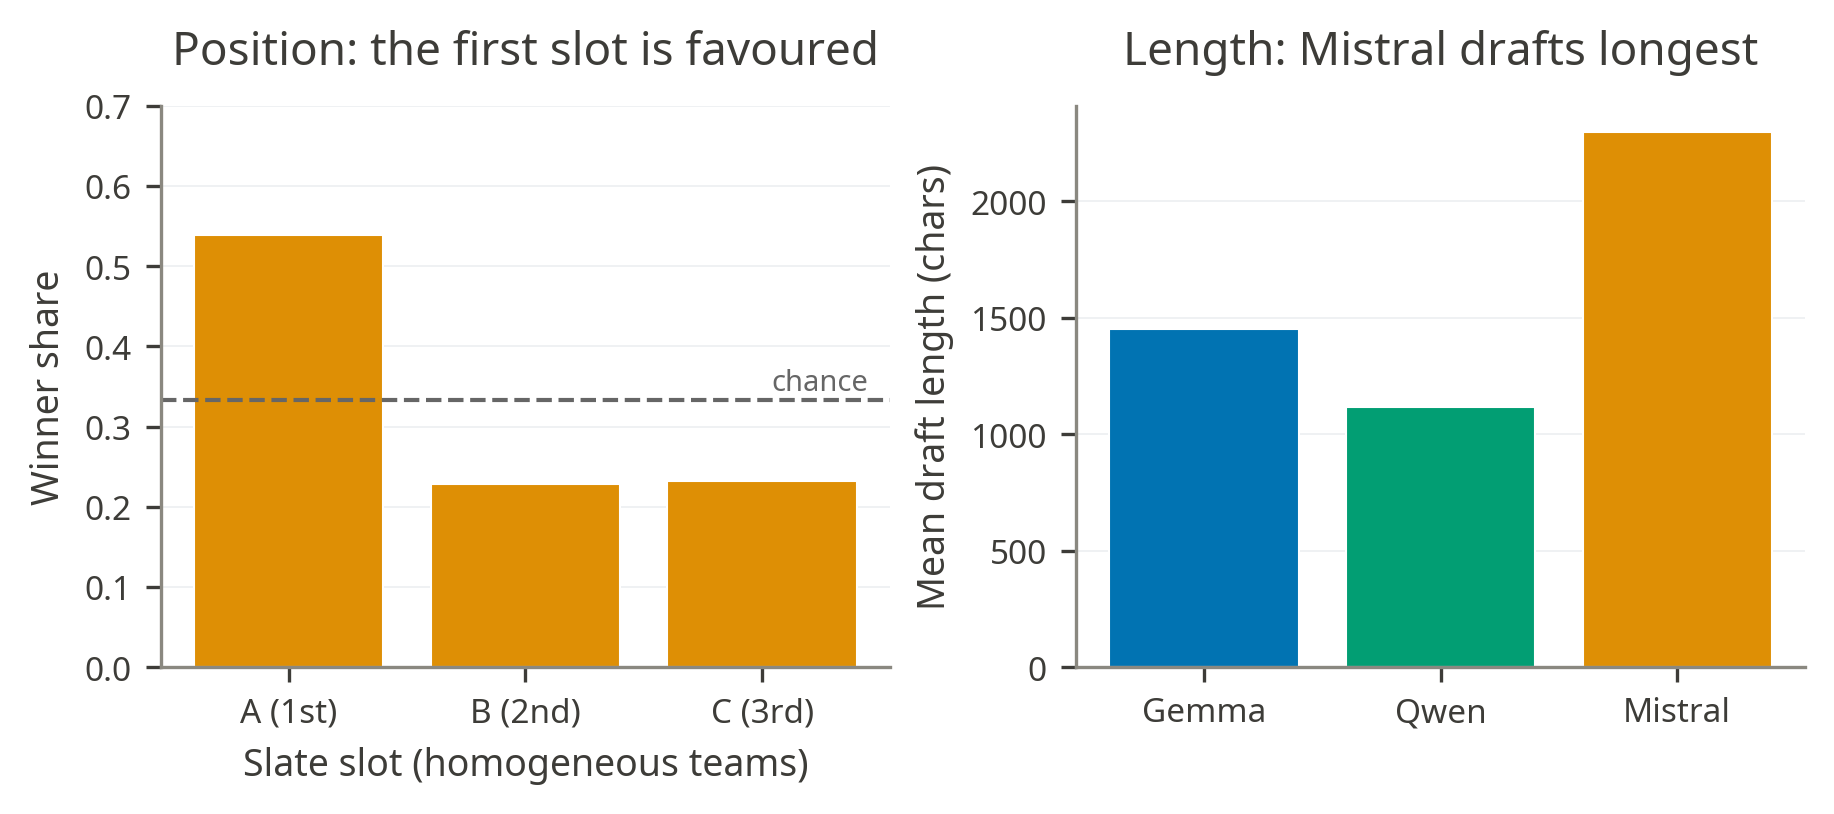
\includegraphics[width=0.95\linewidth]{figures/results/team/consensus_robustness.png}
    \caption{Consensus from homogeneous teams (model held constant).
    Left: winner share by slate slot; the ranking favours the first slot, which Mistral
    never occupies. Right: mean draft length by member in heterogeneous teams; Mistral's
    drafts are the longest, yet within homogeneous teams the longest draft wins only $38\%$
    of votes, near the $33\%$ chance baseline.}
    \label{fig:consensus-robustness}
\end{figure}
